
\section{Acquiring Control System Training Data}

As presented in \secref{patter}, in order for a prosthetic control system to be able to differentiate between movements, a classifier could be trained with EMG data acquired while performing each movement. Therefore, individual subject EMG training data had to be acquired. Training data was acquired using the MYB placed around the thickest part of the dominant forearm while the subject performed wrist pronation, wrist supination, opened hand, closed hand and rest. The subsequent section will document how the data used for training the classifier was acquired. \\
First, a baseline recording was made, where the subject was instructed in keeping the hand perfectly still. The baseline consisted of a 15 second recording and was subtracted from each of the other recordings to reduce baseline noise. If the signal was below the baseline amplitude it was set to zero. \\
During a muscle contraction two main states can be recognized: a transient state, described by inconsistent myoelectric activity as the muscle length is changing, and steady state, where a constant muscle activity is reached. \cite{Mobarak2014} Classification is often based solely on steady state data, however, including transient state might make for a more robust classifier as the delay until steady state is reached is eliminated \cite{Boschmann2013,Mobarak2014a}. \\
%

\begin{figure}[H]                 
	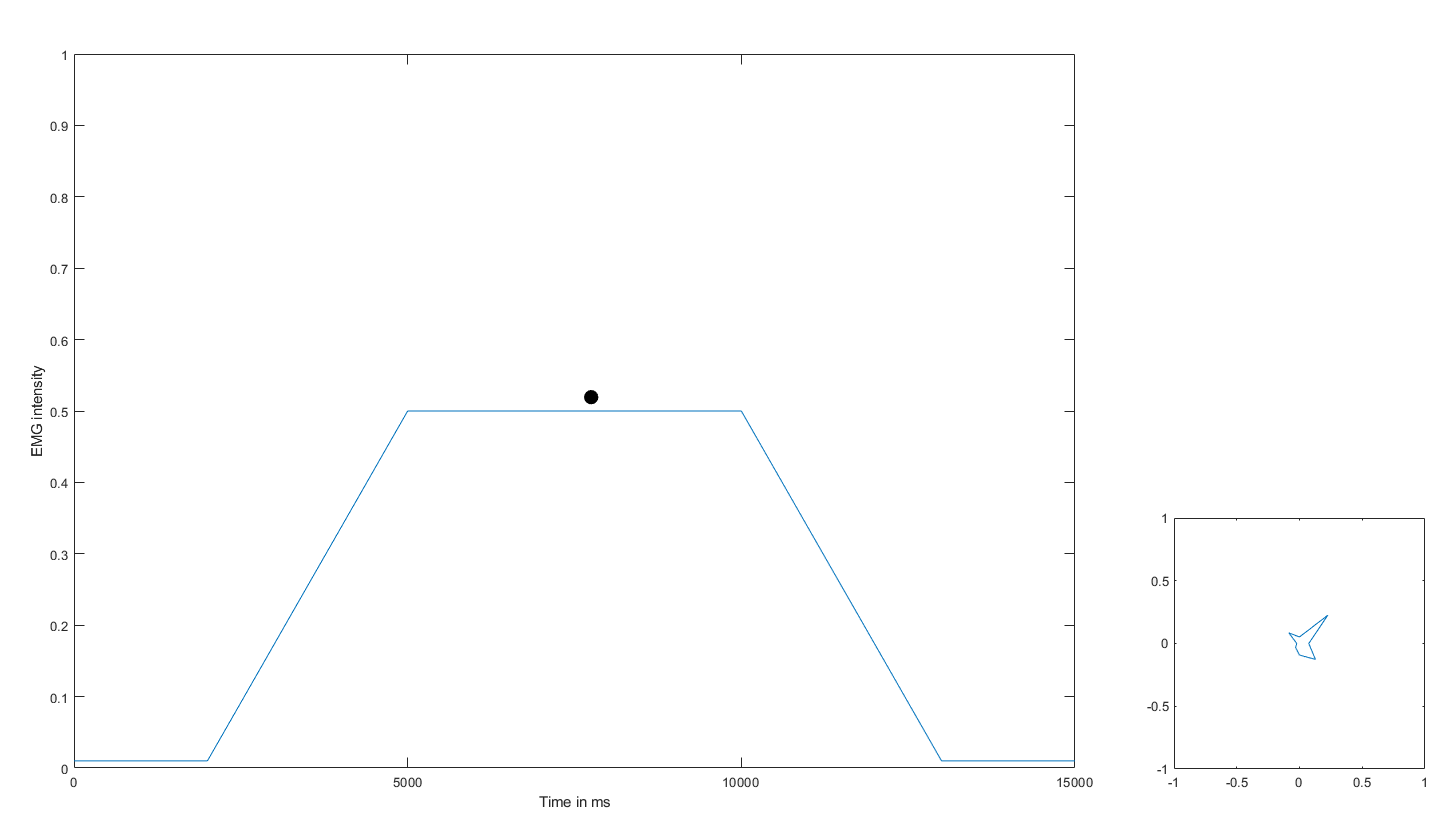
\includegraphics[width=1\textwidth]{figures/trapezoid}  
	\caption{The trapezoidal plot (left) and contraction validation plot (right) used during acquisition of the training data. The trapezoidal plot represented the contraction amplitude requested. The black cursor moved continuous horizontally with time, and the height of the cursor position indicated the currently elicited contraction intensity. The validation plot was used by the investigators to assess the homogeneity of the performed movement. The mean of a segment in each electrode channel was plotted in different directions to get an overview of the activation recorded from the individual channels. The shape of the validation plot should be similar during a recording for it to be homogeneous.}
	\label{fig:GUI} 
\end{figure}
\vspace{-1em}

To feed the classifier with training data representing muscle contractions with varying force, different fractions of maximum contraction force were recorded. In the process of obtaining training data for each movement, the same four contraction were carried out: a prolonged maximum voluntary contraction (pMVC) recording and 40, 50 and 70 $\percent$ of the pMVC recordings.
The pMVC was recorded for 15 seconds where the subject was instructed to elicit the contraction with a maximum contraction force which could be held steady, over the course of the 15 seconds. This resulted in an pMVC for each channel in the MYB, which was calculated as the mean of the absolute values of the EMG signal for each channel. The mean for each channel was used as a maximum reference when acquiring the subsequent fraction recordings. \\
Acquisition of the 40, 50 and 70 $\percent$ fractions of pMVC were done using a graphical user interface (GUI) made in MATLAB 2018b, which can be seen in \figref{fig:GUI}. The image shows the trapezoidal trajectory the subject were instructed to follow using the black cursor, where the height of the cursor was calculated as the mean absolute intensity across all channels of the elicited muscle contraction. The data was extracted over a 200 ms window. The cursor would automatically move positively along the x-axis in relation to time. The high plateau of the trapezoid represented either the 40, 50 and 70 $\percent$ fractions of the pMVC. Data were recorded during 2.5 seconds rest periods in the beginning and end, a 2.5 seconds incline transition, 5 seconds steady state and 2.5 seconds decline transition, summing to a total time of 15 seconds. However, only data recorded during the steady state and the last and first second of the incline and decline of the transition phases, respectively, were used to train the classifier. \\
The additional plot, seen on the right in \figref{fig:GUI}, plotted the amplitude of each of the eight channels in the MYB and was used by the investigators to assess whether the performed movements were done correctly. If the amplitude of the channels responsible for the performed movement shifted rapidly, or if channels not responsible for the performed movement were active, it would indicate that the subject did not perform a correct contraction and the recording would have to be redone.   
   
   
